\chapter{Framework Evaluation and Application}
\label{chapter:application}

To verify that the final version of the framework was effective (see Chapter~\ref{chapter:framework}), I applied it to design a place photo discovery application as well as to reevaluate five of the applications that were used in the construction of the preliminary framework described in Chapter~\ref{chapter:old_framework}. This section outlines application design process, and evaluations of the tools with proposed directions for development of these applications. 

{\section{Application}

{\subsection{KeePlaces}
\begin{figure}[ht!]
	\noindent
	\centering
	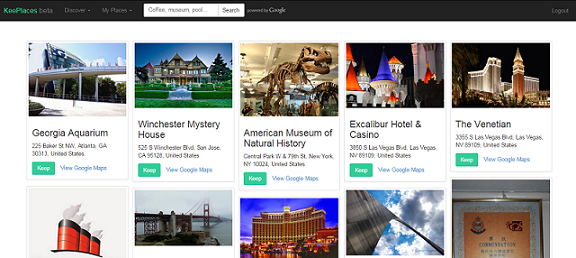
\includegraphics[width=\linewidth]{keeplaces.png}
	\caption{KeePlaces}
	\label{fig:keeplaces} 
\end{figure}
{\subsubsection{Navigation}
Descriptional navigation is possible using search. The search feature is not guided, and so far, results are not personalized. 

}
{\subsubsection{Exploration}
Spatial exploration of multiple resources is enabled through the gallery view. 
Resources are represented as photos, so visual exploration of multiple resources is enabled. However, there is no way of exploring each resource individually, therefore, exploration of a single resource is not supported. 
}
{\subsubsection{Integration}
KeePlaces is integrated with Google Maps.
}
{\subsubsection{Curation}
Curation in Keeplaces is supported through management and preservation.

Management is implemented using collection-based classification.
Every photo discovered on the site can be bookmarked, or 'kept', in a collection.
}
{\subsubsection{Channeling}
Channeling has not yet been enabled within the application, but it is an important aspect behind the conceptual model of the application.
}
{\subsubsection{Directions for Future Development}
As mentioned above, channeling is the first aspect that needs to be implemented along with enhancing management mechanisms.
}
} % end subsection
} % end section



{\section{Final Evaluation}
To illustrate how the framework can be applied to evaluate current Web applications and suggest new tooling, we use it to examine five of the cases of the study.

{\subsection{Pinterest}
Pinterest is an application for image discovery oriented towards finding inspirations and collecting knowledge about hobbies and interest. Resources on Pinterest are called 'pins', collections - 'boards', and users 'pinners'. 

{\subsubsection{Navigation}
Navigation in Pinterest can be accomplished in a few different ways. Descriptional navigation is enabled with a guided search mechanism. However, results of the search are not personalized. 

Referential navigation is accomplished through various implementations. The user can navigate using categories. Through clicking on any of the resources, the user can see related resources. When the user navigates using categories, the system makes further suggestions on subcategories. However, there is not facet-guided navigation or filtering. Furthermore, results and suggestions are not personalized for the user. 

Although there isn't an explicit random navigation mechanism, both descriptional and referential mechanisms usually return novice and serendipitous results to facilitate opportunistic browsing. As mentioned above, results are not personalized.

Finally, Pinterest directly displays information tot he users when they visit the site. Display is personalized and provides results of their own activity history or history and updates from the people they follow.
}% end subsubsection

 
{\subsubsection{Exploration}Exploration mechanisms are extensively taken care of in Pinterst. Multiple resources are represented in a gallery view that, in Pinterest culture, is thought of as a 'pinboard'. Such layout provides good spatial support for exploration and makes it easier to build a mental model by drawing analogies with a real pinboard. 

Single resource does not have a lot of distinct spatial arrangements. However, visually it provides a glimpse into what can be found on he Website that the image came from. Textual preview, however, is limited to the address of the Website.
}% end subsubsection


{\subsubsection{Integration}
Pinterest is integrated with many other Websites and Web applications through visual linking.

}% end subsubsection


{\subsubsection{Curation}

Information management is accomplished through sorting 'pins' into different collections ('boards') thus enabling collection-based classification and internal preservation of internal and external resources. 
}% end subsubsection


Users can upload new 'pins', comment on existing ones, or add descriptions that enable information augmentation. 

Users can also share 'pins' among themselves. 
{\subsubsection{Channeling}
Channeling on Pinterset is accomplished through Following users or individual boards, receiving notifications about their activities, and seeing updates that are directly displayed when users enter the site. 
}% end subsubsection

{\subsubsection{Identified Gaps and Future Prospects}
After applying the framework, it became evident that some of the navigation mechanisms could be supported by personalization of results and personal suggestions.
}% end subsubsection 
} % end subsection


{\subsection{Google Maps}
Google maps is a Web application oriented towards place discovery. It provides services for finding information about places as well as directions.  By answering the questions from the framework, we get the following description of Google Maps.

{\subsubsection{Navigation}
  Any other information discovery must be initiated by search, and thus, the user needs to formulate their information need---the application lacks category-based navigation, so there is nothing that aids users in the formulation of an information need. Once the application returns search results, the possibility for serendipitous information discovery increases.  

Fact finding is well supported in Google Maps. Since the application provides access to only one type of resource (places), there is no need for category-based navigation. Direct navigation is not always possible, but some places are visible on the map so the user can click on a place and the application will display relevant information. Search-based navigation within Google Maps is usually precise and returns accurate search results for specific places. 
}
{\subsubsection{Exploration}
However, the 'reviews' link doesn't have a visual preview to indicate that there are more than just reviews on the linked page. Considering the nature of Google Maps, the semantic of the spatial arrangement of resources is defined by the locations of actual places on the map. More information is presented as a list. 
}
{\subsubsection{Integration}
The application is conveniently integrated with Google+, allowing access to relevant information, such as reviews, images, and hours of operation. Resources are displaced in a uniform fashion making it easy to find information such as addresses and contacts. Some interesting information can be discovered on the business' official Website or integrated Google+ page that the user can navigate to by clicking on 'reviews'.}
{\subsubsection{Curation}There are a few ways to rediscover information through Google Maps. Google Maps employs a history-based revisitation mechanism, so users can see the last few places they searched for when opening the page. Users can bookmark a place on a list called "My Places" by clicking on the 'star' icon. Lastly, it is easy to rediscover information about a place by simply searching for it. Returned results are usually both accurate and reliable.

Google Maps does not allow the creation of custom lists nor does it allow tagging. Users can only bookmark places to the "My Places" list. 

Personal preservation in Google Maps is possible through adding the place to the "My Places" list as mentioned above---by adding internal content to internal storage. Other types of place preservation are possible through Google+, however, not within Google Maps.

Users can evaluate and annotate places through Google+. However, aggregated reviews and ratings are visible on Google Maps. 

It is possible to add a new location to Google Maps. Sharing functionality is limited to the tool providing links and code for embedding.  }
{\subsubsection{Channeling}
Channel-based rediscovery is common among applications with content that is frequently updated. Content provided by Google Maps is fairly stable, and therefore, there are no channel-based discovery mechanisms used by the application.
}% end subsubsection 
{\subsubsection{Identified Gaps and Future Prospects}
Evaluating Google Maps using our conceptual framework helped expose some gaps in its design, so we propose directions for future development. From the description above, it can be estimated that Google Maps' curation mechanisms lack some functionality for public and private curation. Improving public curation mechanisms introduces the possibility of channel-based discovery. Furthermore, adding category-guided navigation mechanisms can help with serendipitous discovery. By no means should an application like that be a replacement to Google Maps. However, it could be oriented towards social discovery and curation, as well as opportunistic place exploration, thereby complimenting the Google Maps application.  
}% end subsubsection 
} % end subsection

{\subsection{Wikipedia}
Wikipedia is an open encyclopedia.

{\subsubsection{Navigation}
Descriptional navigation on Wikipedia is accomplished through search. Results, however, are not personalized to the user, and the search mechanism is not guided by the suggestions of what search terms to use.

Referential mechanisms include a broad category-guided navigation which returns just a few featured articles.

Random navigation provides opportunity to serendipitously discover new articles. 

Wikipedia directly displays featured articles, but the content is, again, not tailored to the user. 
}% end subsubsection 
{\subsubsection{Exploration}
Exploration of multiple resources is very limited. Search results are presented in a list form, and links are represented as text. 
}% end subsubsection 
{\subsubsection{Integration}
Wikipedia is not integrated with other Websites though an occasional section of an article called "External Links". Visual preview is not provided.
}% end subsubsection 
{\subsubsection{Curation}
There is not preservation mechanism available at the site, as well as no management mechanisms. Augmentation is possible through personal contribution to the content of articles.  Sharing of Wikipedia articles is also not supported. 

}% end subsubsection 
{\subsubsection{Channeling}
Information on Wikipedia is curated by various users. Although it is not possible to subscribe to any particular channel, Wikipedia updates featured content that can be viewed on the front page and when navigated to using categories. The users can also see history of recently updates content. 
}% end subsubsection 
{\subsubsection{Identified Gaps and Future Prospects}
It is evident that the biggest gaps in Wikipedia is content curation. 
}% end subsubsection 

} % end subsection


{\subsection{Delicious}
Delicious is a bookmarking application. 

{\subsubsection{Navigation}
In delicious, users can navigate using search (descriptional navigation). Referential navigation is not as developped.

}
{\subsubsection{Exploration}
Exploration for the most part is limited to non-visual factors.
}
{\subsubsection{Integration}
Delicious is integrated with many other Websites through linking. Visual linking is only provided in the "Trending" section of the tool.
}
{\subsubsection{Curation}
Curation is a very important aspect of Delicious. Management is performed through tagging. 

Delicious enables internal preservation of external resources. External sharing of internal resources, as well as adding new resources. 

Information augmentation is possible through tagging and commenting on the added links.
}
{\subsubsection{Channeling}
Channeling is performed thorough subscription mechanisms: users can subscribe to other users and create their networks. 
"Trending" section displays results of social curation, and therefore, enables channel-based discovery.
}
{\subsubsection{Identified Gaps and Future Prospects}
According tot he framework, Delicious lacks visual exploration mechanisms, and certain personalization mechanisms. However, the "Trending" part of the system does provide visual previews and arrange resources in a grid. Although it helps with visual and spatial exploration, at the same time it undermines consistency of resource representation. 
} 
} % end subsection


{\subsection{Yelp}
Yelp is a Web application used to discover local businesses. 

{\subsubsection{Navigation}
Descriptional navigation  is again supported with search-based navigation. 

Referential navigation is enabled using category-based navigation.
}
{\subsubsection{Exploration}
Both visual and spatial exploration is enabled at the site. 
}
{\subsubsection{Integration}
Resources are integrated with Google Maps and with the business Websites. In case of Google Maps, visual integration is applied but not with other links.

}
{\subsubsection{Curation}
Users can bookmark businesses they like within the system. 

Evaluation is possible by rating the businesses. Reviews can also be evaluated by choosing between 'Useful', 'Funny', and 'Cool' metrics.

Users can add resources by writing reviews which also contributes to information augmentation. Users can also ad images of the business. 
}
{\subsubsection{Channeling}
On Yelp, the user can see latest updates from activities of other users. 
}
{\subsubsection{Identified Gaps and Future Prospects}
Identified gaps include lack of management mechanisms when businesses are bookmarked.
}

} % end subsection
} % end section
} % end section